\documentclass{article}
\usepackage{pgfplots}
\pgfplotsset{compat=1.18}

\begin{document}

\begin{figure}[h]
\centering
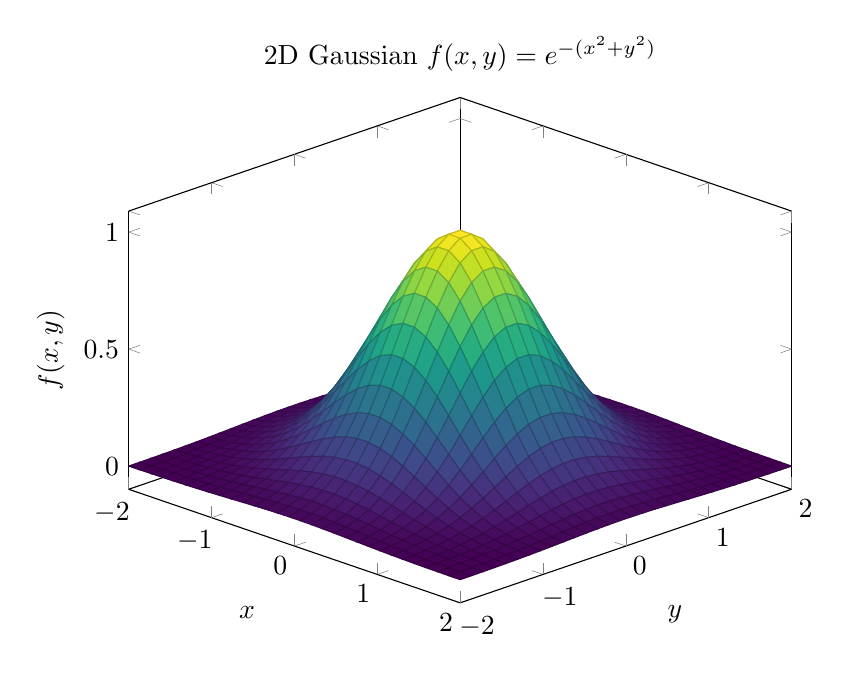
\begin{tikzpicture}
\begin{axis}[
    title={2D Gaussian $f(x,y) = e^{-(x^2+y^2)}$},
    xlabel={$x$},
    ylabel={$y$},
    zlabel={$f(x,y)$},
    view={45}{30},
    colormap/viridis,
    width=10cm,
    height=8cm,
]
\addplot3[
    surf,
    domain=-2:2,
    domain y=-2:2,
    samples=30,
] {exp(-x^2-y^2)};
\end{axis}
\end{tikzpicture}
\caption{A two-dimensional Gaussian surface.}
\label{fig:gaussian}
\end{figure}

\end{document}
